\chapter{Equitable, Clique, and Biclique Coloring}
\label{ch:eq_coloring}

As previously discussed, equitable $k$-colorings seek a coloring of the vertices of an $n$ vertex graph $G$ such that no color is used \say{too many times}. In particular, we want our color classes to have either $\floor{\frac{n}{k}}$ or $\ceil{\frac{n}{k}}$ vertices.
In this chapter, we present a dynamic programming algorithm to handle the problem in chordal graphs, when the number $k$ of colors is fixed, that is, for the \textsc{equitable $k$-coloring} problem.
Moreover, we show that deciding whether or not a block graph $G$ is colorable with $\omega(G)$ colors is $\NPc$ in the strong sense.
Finally, constructive, polynomial time algorithms for \textsc{equitable coloring} on \{net, claw\}-free block graphs, claw-free block graphs and claw-free chordal graphs are presented.

\section{Chordal Graphs}

In this section we will make heavy use of the clique tree $\mathcal{T}(G) = (\mathcal{Q}, F)$ of our chordal graph $G$, which we denote by $\mathcal{T}$ for simplicity.
We also assume that $\mathcal{Q} = \{Q_1, \dots, Q_r\}$, $|V(G)| = n$, that $\mathcal{T}$ is rooted at $Q_1$ and that $T_i$ is the subtree of $\mathcal{T}$ rooted on bag $Q_i$.

Our dynamic programming algorithm explores the separability structure inherent to chordal graphs, embodied by the clique tree, to combine every coloring of a subtree that may yield an equitable coloring of the whole graph.
To do so, we must keep track of which bag, say $Q_i$, we are currently exploring and which colors have been used at the separator between $Q_i$ and $\mathcal{T} \setminus Q_i$.

A \tdef{$k$-color counter}, or simply a \tdef{counter} for an $n$ vertex graph is an element $X \in \left(\left[\ceil{\frac{n}{k}}\right] \cup \{0\}\right)^k$, that is, the $k$-th Cartesian power of $\left[\ceil{\frac{n}{k}}\right] \cup \{0\}$.
A counter $X$ is \tdef{equitable} if for every $x_i, x_j \in X$, $|x_i - x_j| \leq 1$.
For simplicity, denote $S(n,k) = \left[\ceil{\frac{n}{k}}\right] \cup \{0\}$.
The \tdef{sum} of two counters $X,Y$ is defined as $X + Y = (x_1 + y_1, \dots, x_k + y_k)$.
We also define the sum of two families $\mathcal{X}, \mathcal{Y}$ of counters as $\mathcal{Z} = \mathcal{X} + \mathcal{Y} = \left\{X + Y \in S(n,k)^k \mid X \in \mathcal{X}, Y \in \mathcal{Y} \right\}$, that is, the sum of all pairs of elements from each family that belong to $S(n,k)^k$.

\begin{lemma}
    \label{lem:counter_bound}
    If $\mathcal{X}, \mathcal{Y} \subseteq S(n,k)^k$ and $\mathcal{Z} = \mathcal{X} + \mathcal{Y}$, $|\mathcal{Z}| \leq |S(n,k)|^k $.
\end{lemma}

\begin{tproof}
Note that each coordinate of a counter has $|S(n,k)| = \ceil{\frac{n}{k}} + 1$ possible values and, by the definition of the Cartesian product, $|S(n,k)^k| = |S(n,k)|^k$, which implies that $|\mathcal{X}| \leq |S(n,k)|^k$ and $|\mathcal{Y}| \leq |S(n,k)|^k$.
Moreover, every family of counters resulting from the sum of two other families $\mathcal{X}, \mathcal{Y}$ is a subset of $S(n,k)^k$, thus we have that $|\mathcal{Z}| \leq |S(n,k)|^k$.
\end{tproof}


\begin{theorem}
    \label{thm:chordal_exp}
    There is an $\bigO{n^{2k+2}}$ time algorithm for \textsc{equitable $k$-coloring} on chordal graphs.
\end{theorem}

\begin{tproof}
    Let $G$ be the input chordal graph of order $n$ and $\mathcal{T}$ its clique tree, rooted at bag $Q_1$. Moreover, we assume that $k \geq \omega(G)$, otherwise the answer is trivially $\NOi$.
    
    For a bag $Q$, denote by $p(Q)$ the parent clique of $Q$ on $\mathcal{T}$, $I(Q) = Q \cap p(Q)$ and by $U(Q) = Q \setminus p(Q)$ the set of vertices that first appeared on the path between $Q$ and the root $Q_1$ (if $Q = Q_1$, $U(Q) = Q$).
    
    Given $Q$ and a list of available colors $L$, define $\Pi(Q,L)$ as the set of all colorings of $U(Q)$ using only the colors of $L$, $\beta(Q,L,\pi)$ the list of colors used by $L$ and $\pi$ to color $I(Q)$ and $Y(Q,\pi)$ as the counter where $y_i = 1$ if and only if some vertex of $U(Q)$ was colored with color $i$ in $\pi$.
    
    We define our dynamic programming state $f(Q_i, L)$ as all colorings of $T_i$ conditioned to the fact that $I(Q_i)$ was colored with $L$. Intuitively, we will try every possible coloring $\pi$ of $U(Q)$ and combine the solutions of each bag adjacent to $Q_i$ given the colors used by $\pi$ and $L$. Finally, there will be an equitable $k$-coloring of $G$ if there is an equitable counter in $f(Q_1, \emptyset)$.
    
    \begin{equation*}
        f(Q_i, L) = \bigcup_{\pi \in \Pi(Q_i, [k] \setminus L)} \left(Y(Q_i, \pi) + \sum_{Q_j \in N_{T_i}(Q_i)} f(Q_j, \beta(Q_j, L, \pi))\right)
    \end{equation*}
    
    To prove the correctness of our algorithm, we will use induction on the size of $\mathcal{T}$.
    For the base case, where $|V(\mathcal{T})| = 1$, trivially, any proper coloring of $G$ will be equitable.
    
    For the general case, suppose that $Q_i$ has at least one child, say $Q_j$.
    Inductively, for any list of colors $R$, $f(Q_j, R)$ holds every proper coloring of $T_j \setminus I(Q_j)$, given that $I(Q_j)$ was colored with $R$.
    In particular, for every $\pi \in \Pi(Q_i, [k] \setminus L)$ we have this guarantee.
    Note that, for each pair of children $Q_j, Q_l$ of $Q_i$, their solutions are completely independent because $Q_j \cap Q_l \subseteq Q_i$ (clique tree property) and $Q_i$ is entirely colored by $\pi$ and $L$.
    This implies that no vertex was counted more than once on each counter, since their color is chosen exactly once for each possible $\pi$.
    Therefore, since the problems are independent for each child of $Q_i$, $\mathcal{Z}(\pi) = \sum_{Q_j \in N_{T_i}(Q_i)} f(Q_j, \beta(Q_j, L, \pi))$ combines every possible coloring of the children of $Q_i$ and $\mathcal{Z}(\pi) + Y(Q_i, \pi)$ is the family of all colorings of $T_i$, given that $Q_i$ was colored with $\pi$ and $L$.
    Finally, $\bigcup_{\pi \in \Pi(Q_i, [k] \setminus L)} Y(Q, \pi) + Z(\pi)$ tries every possible coloring $\pi$ of $Q_i$, guaranteeing that $f(Q_i, L)$ has every possible coloring of $T_i$, given that $I(Q_i)$ used $L$.
    Since $f(Q_i, L)$ has every coloring of $\mathcal{T_i}$ given $L$, $G$ will be equitably $k$-colorable if and only if there is an equitable counter at $f(Q_1, \emptyset)$.
    
    In terms of complexity analysis, we first note that each sum of two counter families $\mathcal{X},\mathcal{Y}$ takes $\bigO{|\mathcal{X}||\mathcal{Y}|}$.
    However, due to Lemma~\ref{lem:counter_bound}, the size of $\mathcal{X} + \mathcal{Y}$ is at most $|S(N,k)|^k$ and, therefore, $\sum_{Q_j \in N_{T_i}(Q_i)} f(Q_j, \beta(Q_j, L, \pi))$ takes at most $\bigO{n|S(n,k)|^{2k}} = \bigO{n \left(\ceil{\frac{n}{k}} + 1\right)^{2k}}$ time; moreover, the addition of $Y(Q_i, \pi)$ to $\mathcal{Z}(\pi)$, by the same argument, is $\bigO{|S(n,k)|^k}$.
    
    For the outermost union, we have $\bigO{k!}$ possible colorings $\pi$ for $U(Q_i)$, which implies that computing each $f(Q_i, L)$ takes $\bigO{k!n\left(\ceil{\frac{n}{k}} + 1\right)^{2k}}$ time.
    Since we have $r \leq n$ bags and $k!$ possible lists, there are $\bigO{nk!}$ states, therefore the total complexity of our dynamic programming algorithm is $\bigO{k!^2n^2\left(\ceil{\frac{n}{k}} + 1\right)^{2k}} = \bigO{n^{2k + 2}}$.
\end{tproof}

\begin{corollary}
    \textsc{equitable $k$-coloring} of chordal graphs parameterized by the number of colors is in $\XP$.
\end{corollary}


We also have a dynamic programming algorithm with a very similar running time for block graphs; however, their simpler structure appears to only reduce the size of each state.
That is, instead of storing $f(Q, L)$, which has $\bigO{k!n}$ possibilities, we are only required to store a single color, as the interface between cliques on the clique tree is a single vertex.
We omit the algorithm for brevity.

In terms of the effective complexity, the $\NPcness$ of \textsc{equitable coloring} of chordal graphs has been known for some time, since interval graphs are chordal graphs and $\NPcness$ of the problem for this class was proven by~\citep{graph_partitioning1}.


\section{Block Graphs}
\label{sec:blocks}

Despite previous results in the literature pointing that \textsc{equitable coloring} of chordal graphs is $\NPc$, there are some known subclasses that had not been dealt with; in particular, block graphs.
Before showing that \textsc{equitable coloring} of block graphs is $\NPc$, we first define a key gadget for our reduction, which we call \tdef{(a,k)-flower}.

\begin{definition}[$(a,k)$-flower]
    Let $a,k$ be positive integers. An $(a,k)$-flower $F(a,k)$ is defined as $F(a,k) = K_1 \oplus \bigcup_{i \leq a+1} K_{k-1}$, that is, the join of a single vertex with the disjoint union of $a+1$ cliques of size $k-1$.
\end{definition}

\begin{figure}[!htb]
    \centering
    \begin{tikzpicture}[scale=1]
        %\draw[help lines] (-5,-5) grid (5,5);
        \GraphInit[unit=3,vstyle=Normal]
        \SetVertexNormal[Shape=circle, FillColor=black, MinSize=2pt]
        \tikzset{VertexStyle/.append style = {inner sep = \inners, outer sep = \outers}}
        \SetVertexNoLabel
        \Vertex[x=0,y=0,L={y}, Lpos=270, LabelOut, Ldist=3pt]{y}
        \Vertex[a=-5, d=1.7cm]{x11}
        \Vertex[a=-30, d=2.3cm]{x12}
        \Vertex[a=-55, d=1.7cm]{x13}
        
        \Vertex[a=115, d=1.7cm]{x21}
        \Vertex[a=90, d=2.3cm]{x22}
        \Vertex[a=65, d=1.7cm]{x23}
        
        \Vertex[a=235, d=1.7cm]{x31}
        \Vertex[a=210, d=2.3cm]{x32}
        \Vertex[a=185, d=1.7cm]{x33}
        
        \foreach \x in {1,2,3}
            \foreach \y in {1,2,3}
                \Edge(y)(x\x\y);
        
        \Edge(x11)(x12)
        \Edge(x11)(x13)
        \Edge(x12)(x13)
        
        
        \Edge(x21)(x22)
        \Edge(x21)(x23)
        \Edge(x22)(x23)
        
        
        \Edge(x31)(x32)
        \Edge(x31)(x33)
        \Edge(x32)(x33)
        
        
    \end{tikzpicture}
    
    \caption{A $(2,4)$-flower.}
    \label{fig:flower}
\end{figure}

Note that each $(a,k)$-flower is a block graph with a single cut vertex and a collection of $a+1$ cliques of size $k$ each.

\begin{theorem}
    \label{thm:disc_block_npc}
    \textsc{equitable coloring} of block graphs is $\NPc$.
\end{theorem}

\begin{tproof}
    We will perform a reduction from the \textsc{bin-packing} problem, a known partitioning problem, which is $\NPc$ in the strong sense (problem SR1 of~\citep{garey_johnson}).
    
    \problem{bin-packing}{Integers $A = \{a_1, \dots, a_n\}$, a bin capacity $B$ and a number of bins $k$.}{Is there a $k$-partition $\varphi$ of $A$ such that for every bin $i$, $\sum_{a_j \in \varphi_i} a_j = B$?}
    
    Our instance of \textsc{equitable coloring} is given by $G = \bigcup_{a_j \in A} F(a_j,k)$, that is, the disjoint union of $n$ flowers, one for each element of $A$, and we ask for an equitable $k$-coloring of $G$.
    For simplicity, we denote $F(a_j, k)$ by $F_j$ and by $y_j$ the cut vertex of $F_j$.
    Note that
    
    \begin{align*}
        |V(G)| &= \sum_{j \in [n]} |V(F_j)|\\
               &= \sum_{j \in [n]} \left((a_j + 1)(k-1) + 1\right)\\
               &= (k-1)\left(n + \sum_{j \in [n]} a_j\right) + n\\
               &= (k-1)(n + kB) + n\\
               &= kn + k^2B - n - kB + n\\
               &= k(kB - B + n)
    \end{align*}
    
    Suppose that we are given a $k$-partition $\varphi$ of $A$ that solves the problem.
    We build a $k$-coloring $\psi$ of $G$ such that $\psi(y_j) = i$ if $a_j \in \varphi_i$.
    The remaining vertices of each $F_j$ have a single possible proper coloring, since $y_j$ is universal in $F_j$ and each one of the $a_j + 1$ cliques with $k-1$ vertices have exactly $k-1$ available colors to be used. Therefore, each color class $\psi_i$ satisfies the following equality and $\psi$ is an equitable $k$-coloring.
    
    \begin{align*}
        |\psi_i| &= |\varphi_i| + \sum_{j \mid y_j \notin \psi_i} (a_j + 1)\\
                 &= |\varphi_i| + \sum_{j \in [n]} (a_j + 1) - \sum_{j \mid y_j \in \psi_i} (a_j + 1)\\
                 &= |\varphi_i| + n + kB - B - |\varphi_i|\\
                 &= kB - B + n = \frac{|V(G)|}{k}
    \end{align*}
    
    
    For the converse, take an equitable $k$-coloring $\psi$ of $G$, and build a $k$-partition $\varphi$ of $A$ such that $a_j \in \varphi_i$ if $\psi(y_j) = i$.
    It remains to prove that every bin $i$ satisfies $\sum_{a_j \in \varphi_i} a_j = B$.
    The following equalities give this guarantee and complete the proof.
    
    \begin{align*}
        kB - B + n &= |\psi_i|\\
                   &= \sum_{j \mid y_j \in \psi_i} 1 + \sum_{j \mid y_j \notin \psi_i} (a_j + 1)\\
                   &= \sum_{j \mid y_j \in \psi_i} 1 + \sum_{j \in [n]} (a_j + 1) - \sum_{j \mid y_j \in \psi_i} (a_j + 1) \\
                   &= kB + n - \sum_{j \mid y_j \in \psi_i} a_j\\
            B      &= \sum_{j \mid y_j \in \psi_i} a_j
    \end{align*}
\end{tproof}

In terms of parameterized complexity, \textsc{bin-packing} is $\W[1]\text{-}\Hard$ parameterized by the number of bins~\citep{bin_packing_w1}.
Moreover, the graph built on the proof of Theorem~\ref{thm:disc_block_npc} is also a cograph since it is $P_4$-free.
These observations allow us to obtain the following corollaries.

\begin{corollary}
    \textsc{equitable coloring} of graphs that are chordal graphs and cographs is $\NPc$.
\end{corollary}

\begin{corollary}
    \textsc{equitable coloring} of graphs that are chordal grapjs and cographs parameterized by the number of colors is $\W[1]\text{-}\Hard$.
\end{corollary}

The next theorem uses a slight variation of the proof of Theorem~\ref{thm:disc_block_npc} to show that hardness remains for block graphs with diameter equal to 5.
That is, even with relatively few choices to be performed, the task is still complicated.

\begin{figure}[!htb]
    \centering
    \begin{tikzpicture}[scale=1]
            %\draw[help lines] (-8,-8) grid (8,8);
        \begin{scope}[rotate=36,shift={(0cm, 5cm)}]
            \GraphInit[unit=3,vstyle=Normal]
            \SetVertexNormal[Shape=circle, FillColor=black, MinSize=2pt]
            \tikzset{VertexStyle/.append style = {inner sep = \inners, outer sep = \outers}}
            \SetVertexNoLabel
            \Vertex[Math, x=0,y=0,L={y_1}, Lpos=290, LabelOut, Ldist=3pt]{1y}
            \Vertex[a=-5, d=1.7cm]{1x11}
            \Vertex[a=-30, d=2.3cm]{1x12}
            \Vertex[a=-55, d=1.7cm]{1x13}
            
            \Vertex[a=115, d=1.7cm]{1x21}
            \Vertex[a=90, d=2.3cm]{1x22}
            \Vertex[a=65, d=1.7cm]{1x23}
            
            \Vertex[a=235, d=1.7cm]{1x31}
            \Vertex[a=210, d=2.3cm]{1x32}
            \Vertex[a=185, d=1.7cm]{1x33}
            
            \foreach \x in {1,2,3}
                \foreach \y in {1,2,3}
                    \Edge(1y)(1x\x\y);
            
            \Edge(1x11)(1x12)
            \Edge(1x11)(1x13)
            \Edge(1x12)(1x13)
            
            
            \Edge(1x21)(1x22)
            \Edge(1x21)(1x23)
            \Edge(1x22)(1x23)
            
            
            \Edge(1x31)(1x32)
            \Edge(1x31)(1x33)
            \Edge(1x32)(1x33)
        \end{scope}
        \begin{scope}[rotate=-36,shift={(0cm, 5cm)}]
            \GraphInit[unit=3,vstyle=Normal]
            \SetVertexNormal[Shape=circle, FillColor=black, MinSize=2pt]
            \tikzset{VertexStyle/.append style = {inner sep = \inners, outer sep = \outers}}
            \SetVertexNoLabel
            \Vertex[Math, x=0,y=0,L={y_1}, Lpos=290, LabelOut, Ldist=3pt]{2y}
            \Vertex[a=-5, d=1.7cm]{2x11}
            \Vertex[a=-30, d=2.3cm]{2x12}
            \Vertex[a=-55, d=1.7cm]{2x13}
            
            \Vertex[a=115, d=1.7cm]{2x21}
            \Vertex[a=90, d=2.3cm]{2x22}
            \Vertex[a=65, d=1.7cm]{2x23}
            
            \Vertex[a=235, d=1.7cm]{2x31}
            \Vertex[a=210, d=2.3cm]{2x32}
            \Vertex[a=185, d=1.7cm]{2x33}
            
            \foreach \x in {1,2,3}
                \foreach \y in {1,2,3}
                    \Edge(2y)(2x\x\y);
            
            \Edge(2x11)(2x12)
            \Edge(2x11)(2x13)
            \Edge(2x12)(2x13)
            
            
            \Edge(2x21)(2x22)
            \Edge(2x21)(2x23)
            \Edge(2x22)(2x23)
            
            
            \Edge(2x31)(2x32)
            \Edge(2x31)(2x33)
            \Edge(2x32)(2x33)
        \end{scope}
        \begin{scope}[rotate=-108,shift={(0cm, 5cm)}]
            \GraphInit[unit=3,vstyle=Normal]
            \SetVertexNormal[Shape=circle, FillColor=black, MinSize=2pt]
            \tikzset{VertexStyle/.append style = {inner sep = \inners, outer sep = \outers}}
            \SetVertexNoLabel
            \Vertex[Math, x=0,y=0,L={y_1}, Lpos=290, LabelOut, Ldist=3pt]{3y}
            \Vertex[a=-5, d=1.7cm]{3x11}
            \Vertex[a=-30, d=2.3cm]{3x12}
            \Vertex[a=-55, d=1.7cm]{3x13}
            
            \Vertex[a=115, d=1.7cm]{3x21}
            \Vertex[a=90, d=2.3cm]{3x22}
            \Vertex[a=65, d=1.7cm]{3x23}
            
            \Vertex[a=235, d=1.7cm]{3x31}
            \Vertex[a=210, d=2.3cm]{3x32}
            \Vertex[a=185, d=1.7cm]{3x33}
            
            \foreach \x in {1,2,3}
                \foreach \y in {1,2,3}
                    \Edge(3y)(3x\x\y);
            
            \Edge(3x11)(3x12)
            \Edge(3x11)(3x13)
            \Edge(3x12)(3x13)
            
            
            \Edge(3x21)(3x22)
            \Edge(3x21)(3x23)
            \Edge(3x22)(3x23)
            
            
            \Edge(3x31)(3x32)
            \Edge(3x31)(3x33)
            \Edge(3x32)(3x33)
        \end{scope}
        \begin{scope}[rotate=108,shift={(0cm, 5cm)}]
            \GraphInit[unit=3,vstyle=Normal]
            \SetVertexNormal[Shape=circle, FillColor=black, MinSize=2pt]
            \tikzset{VertexStyle/.append style = {inner sep = \inners, outer sep = \outers}}
            \SetVertexNoLabel
            \Vertex[Math, x=0,y=0,L={y_1}, Lpos=290, LabelOut, Ldist=3pt]{4y}
            \Vertex[a=-5, d=1.7cm]{4x11}
            \Vertex[a=-30, d=2.3cm]{4x12}
            \Vertex[a=-55, d=1.7cm]{4x13}
            
            \Vertex[a=115, d=1.7cm]{4x21}
            \Vertex[a=90, d=2.3cm]{4x22}
            \Vertex[a=65, d=1.7cm]{4x23}
            
            \Vertex[a=235, d=1.7cm]{4x31}
            \Vertex[a=210, d=2.3cm]{4x32}
            \Vertex[a=185, d=1.7cm]{4x33}
            
            \foreach \x in {1,2,3}
                \foreach \y in {1,2,3}
                    \Edge(4y)(4x\x\y);
            
            \Edge(4x11)(4x12)
            \Edge(4x11)(4x13)
            \Edge(4x12)(4x13)
            
            
            \Edge(4x21)(4x22)
            \Edge(4x21)(4x23)
            \Edge(4x22)(4x23)
            
            
            \Edge(4x31)(4x32)
            \Edge(4x31)(4x33)
            \Edge(4x32)(4x33)
        \end{scope}
        \begin{scope}[rotate=120,shift={(0cm, 0cm)}]
            \GraphInit[unit=3,vstyle=Normal]
            \SetVertexNormal[Shape=circle, FillColor=black, MinSize=2pt]
            \tikzset{VertexStyle/.append style = {inner sep = \inners, outer sep = \outers}}
            \SetVertexNoLabel
            \Vertex[Math, x=0,y=0,L={y_1}, Lpos=290, LabelOut, Ldist=3pt]{0y}
            \Vertex[a=-15, d=1.7cm]{0x11}
            \Vertex[a=-30, d=2.3cm]{0x12}
            \Vertex[a=-45, d=1.7cm]{0x13}
            
            \Vertex[a=-87, d=1.7cm]{0x21}
            \Vertex[a=-102, d=2.3cm]{0x22}
            \Vertex[a=-117, d=1.7cm]{0x23}
            
            \Vertex[a=-159, d=1.7cm]{0x31}
            \Vertex[a=-174, d=2.3cm]{0x32}
            \Vertex[a=-189, d=1.7cm]{0x33}
            
            \Vertex[a=-231, d=1.7cm]{0x41}
            \Vertex[a=-246, d=2.3cm]{0x42}
            \Vertex[a=-261, d=1.7cm]{0x43}
            
            \Vertex[a=-303, d=1.7cm]{0x51}
            \Vertex[a=-318, d=2.3cm]{0x52}
            \Vertex[a=-333, d=1.7cm]{0x53}
            
            
            \foreach \x in {1,2,3,4,5}
                \foreach \y in {1,2,3}
                    \Edge(0y)(0x\x\y);
                    
                    \Edge(0x11)(0x11)
            \Edge(0x11)(0x12)
            \Edge(0x11)(0x13)
            \Edge(0x12)(0x12)
            \Edge(0x12)(0x13)
            \Edge(0x13)(0x13)
            \Edge(0x21)(0x21)
            \Edge(0x21)(0x22)
            \Edge(0x21)(0x23)
            \Edge(0x22)(0x22)
            \Edge(0x22)(0x23)
            \Edge(0x23)(0x23)
            \Edge(0x31)(0x31)
            \Edge(0x31)(0x32)
            \Edge(0x31)(0x33)
            \Edge(0x32)(0x32)
            \Edge(0x32)(0x33)
            \Edge(0x33)(0x33)
            \Edge(0x41)(0x41)
            \Edge(0x41)(0x42)
            \Edge(0x41)(0x43)
            \Edge(0x42)(0x42)
            \Edge(0x42)(0x43)
            \Edge(0x43)(0x43)
            \Edge(0x51)(0x51)
            \Edge(0x51)(0x52)
            \Edge(0x51)(0x53)
            \Edge(0x52)(0x52)
            \Edge(0x52)(0x53)
            \Edge(0x53)(0x53)
            
        \end{scope}
        \Edge(0y)(1y)
        \Edge(0y)(2y)
        \Edge(0y)(3y)
        \Edge(0y)(4y)
        
        
    \end{tikzpicture}
    
    \caption{\textsc{equitable coloring} instance built on Theorem~\ref{thm:diam_block} corresponding to the \textsc{bin-packing} instance $A = \{2,2,2,2\}$, $k=3$ and $B = 4$.}
    \label{fig:super_flower}
\end{figure}


\begin{theorem}
    \label{thm:diam_block}
    \textsc{equitable coloring} of block graphs with diameter equal to 4 is $\NPc$.
\end{theorem}

\begin{tproof}
    For this proof, we also perform a reduction from \textsc{bin-packing}, but use one extra flower $F(B, k+1)$, which we denote by $F_0$, with $y_0$ being its cut-vertex.
    Our instance is given by a graph $G$ with $V(G) = V(F(B, k+1)) \cup \bigcup_{j \leq n} V(F(a_j, k+1))$, $E(G) = \{y_0y_j \mid j \leq n\} \cup E(F(B, k+1)) \cup \bigcup_{j \leq n} E(F(a_j, k+1))$ and we attempt to equitably $(k+1)$-color $G$, which satisfies
    
    \begin{align*}
        |V(G)| &= |V(F_0)| + \sum_{j \in [n]} |V(F_j)|\\
               &= k(B + 1) + 1 + \sum_{j \in [n]} \left(1 + k(a_j + 1)\right)\\
               &= kB + k + n + k^2B + kn + 1\\ 
               &= (k+1)(kB + n + 1)
    \end{align*}
    
    Given a $k$-partition $\varphi$ of $A$ that solves our instance of \textsc{bin-packing}, we construct a coloring $\psi$ of $G$ such that $\psi(y_j) = i$ if $a_j \in \varphi_i$ and $\psi(y_0) = k+1$.
    Using a similar argument to the previous theorem, after coloring each $y_j$, the remaining vertices of $G$ are automatically colored.
    For $\psi_{k+1}$, it is easy to see that $|\psi_{k+1}| = 1 + \sum_{j \in [n]} (a_j + 1) = kB + n + 1 = \frac{|V(G)|}{k+1}$.
    It remains to prove that every other color class $\psi_i$ also has $\frac{|V(G)|}{k+1}$ vertices.
    
    \begin{align*}
        |\psi_i| &= B + 1 + \sum_{j \mid y_j \notin \psi_i} (a_j + 1) + \sum_{j \mid y_j \in \psi_i} 1\\
                 &= B + 1 + \sum_{j \in [n]} (a_j + 1) - \sum_{j \mid y_j \in \psi_i} (a_j + 1) + \sum_{j \mid y_j \in \psi_i} 1\\
                 &= B + 1 + kB + n - B\\
                 &= kB + n + 1
    \end{align*}
    
    For the converse we take an equitable $(k+1)$-coloring of $G$ and suppose, without loss of generality, that $\psi(y_0) = k+1$ and, consequently, for every other $y_i$, $\psi(y_i) \neq k+1$.
    To build our $k$-partition $\varphi$ of $A$, we say that $a_j \in \varphi_i$ if $\psi(y_j) = i$.
    The following equalities show that $\sum_{a_j \in \varphi_i} a_j = B$ for every $i$ and completes the proof.
    
    \begin{align*}
        kB + n + 1 &= |\psi_i|\\
                   &= B + 1 + \sum_{j \mid y_j \in \psi_i} 1 + \sum_{j \mid y_j \notin \psi_i} (a_j + 1)\\
                   &= B + 1 + \sum_{j \mid y_j \in \psi_i} 1 + \sum_{j \in [n]} (a_j + 1) - \sum_{j \mid y_j \in \psi_i} (a_j + 1) \\
                   &= B + 1 + kB + n - \sum_{j \mid y_j \in \psi_i} a_j \\
                 0 &= B - \sum_{j \mid y_j \in \psi_i} a_j
    \end{align*}
\end{tproof}

\section{Claw-free graphs}

In this section we explore some properties of claw-free graphs, in particular, subclasses of chordal graphs, that enable us to give constructive algorithms for these classes.
These results complement de Werra's (indirect) theorem that every claw-free graph $G$ admits an equitable $k$-coloring for $k \geq \chi(G)$.
We begin with a very simple class and increase its complexity, along with the corresponding algorithm's, until we have a result for claw-free chordal graphs.
For the entirety of this section, we will assume that our colorings are \tdef{contiguous}, that is, the colored vertices of $G$, given a partial equitable coloring $\varphi$ of $G$, induce a connected subgraph of $G$.

\subsection{\{net, claw\}-free Block Graphs}

\begin{figure}[!htb]
    \centering
    \begin{tikzpicture}[scale=1]
        \begin{scope}
            %\draw[help lines] (-5,-5) grid (5,5);
            \GraphInit[unit=3,vstyle=Normal]
            \SetVertexNormal[Shape=circle, FillColor=black, MinSize=2pt]
            \tikzset{VertexStyle/.append style = {inner sep = \inners, outer sep = \outers}}
            \SetVertexNoLabel
            \Vertex[a=90, d=1cm]{a}
            \Vertex[a=210, d=1cm]{b}
            \Vertex[a=330, d=1cm]{c}
            \Vertex[a=90, d=2cm]{a2}
            \Vertex[a=210, d=2cm]{b2}
            \Vertex[a=330, d=2cm]{c2}
            
            \Edge(a)(a2)
            \Edge(b)(b2)
            \Edge(c)(c2)
            \Edge(a)(b)
            \Edge(a)(c)
            \Edge(b)(c)
        \end{scope}
    \end{tikzpicture}
    \hfill
    \begin{tikzpicture}[scale=1]
        \begin{scope}[rotate=90]
            %\draw[help lines] (-5,-5) grid (5,5);
            \GraphInit[unit=3,vstyle=Normal]
            \SetVertexNormal[Shape=circle, FillColor=black, MinSize=2pt]
            \tikzset{VertexStyle/.append style = {inner sep = \inners, outer sep = \outers}}
            \SetVertexNoLabel
            \grStar[RA=2]{4}
        \end{scope}
    \end{tikzpicture}
    \hfill
    \begin{tikzpicture}[scale=1]
        \begin{scope}[shift={(0.5cm,-4cm)},scale=0.9]
            %\draw[help lines] (-5,-5) grid (5,5);
            \begin{scope}[shift={(-4cm, 0cm)}]
                \GraphInit[unit=3,vstyle=Normal]
                \SetVertexNormal[Shape=circle, FillColor=black, MinSize=2pt]
                \tikzset{VertexStyle/.append style = {inner sep = \inners, outer sep = \outers}}
                \SetVertexNoLabel
                \grComplete[RA=1]{5}
            \end{scope}
            \begin{scope}[rotate=-30,shift={(-2.105cm,-0.64cm)}]
                \GraphInit[unit=3,vstyle=Normal]
                \SetVertexNormal[Shape=circle, FillColor=black, MinSize=2pt]
                \tikzset{VertexStyle/.append style = {inner sep = \inners, outer sep = \outers}}
                \SetVertexNoLabel
                \grComplete[RA=1]{3}
            \end{scope}
            \begin{scope}[shift={(-0.295cm, 0cm)}]
                \GraphInit[unit=3,vstyle=Normal]
                \SetVertexNormal[Shape=circle, FillColor=black, MinSize=2pt]
                \tikzset{VertexStyle/.append style = {inner sep = \inners, outer sep = \outers}}
                \SetVertexNoLabel
                \grComplete[RA=1]{6}
            \end{scope}
            \begin{scope}[rotate=180,shift={(-1.705cm, 0cm)}]
                \GraphInit[unit=3,vstyle=Normal]
                \SetVertexNormal[Shape=circle, FillColor=black, MinSize=2pt]
                \tikzset{VertexStyle/.append style = {inner sep = \inners, outer sep = \outers}}
                \SetVertexNoLabel
                \grComplete[RA=1]{5}
            \end{scope}
        \end{scope}
    \end{tikzpicture}
    \hfill
    
    
    \caption{A net (left), a claw (center) and a \{net, claw\}-free block graph (right).}
    \label{fig:net_claw}
\end{figure}

The first subclass we study are exactly the \tdef{\{net, claw\}-free block graphs}, to which we find a polynomial time algorithm for the problem.
A \tdef{net} is a cycle of size 3 with one adjacent vertex to each vertex of the cycle; a \tdef{claw} is a star $K_{1,3}$.
Essentially, \{net, claw\}-free block graphs are a sequence of cliques $Q_1, \dots, Q_r$, with each clique having at most two cut vertices.

\begin{theorem}
    \label{thm:fat_path}
    There is a polynomial time algorithm for \textsc{equitable coloring} restricted to \{net, claw\}-free block graphs.
\end{theorem}

\begin{tproof}
    Let $G$ be our \{net, claw\}-free block graph of order $n$, $k \geq \omega(G)$ and suppose we have an ordering $Q_1, \dots, Q_r$ of the cliques of $G$.
    Our algorithm greedily colors the non cut-vertices of the current clique of the sequence and, when there are none remaining, colors the cut-vertex, if it exists.
    
    We prove by induction on $r$ that the last clique of the sequence always has at least one vertex colored with one of the $l$ most frequently used colors.
    The base case is a single clique, which trivially admits an equitable $k$-coloring and every vertex has one of the most frequently used colors.
    For general $r > 1$, we have that $G[Q_1, \dots, Q_{r-1}]$ has an equitable $k$-coloring and that at least one vertex of $Q_{r-1}$ is colored with one of the $l$ most frequently used colors.
    Clearly, the cut vertex $y_{r-2}$ (if it exists) between $Q_{r-2}$ and $Q_{r-1}$ cannot be the only one colored with such a color, since $Q_{r-1}$ was colored after it.
    Therefore, any coloring of $Q_{r-1} \setminus y_{r-2}$ can be rearranged such that the next cut vertex, $y_{r-1}$ has one of the $l$ most frequent colors.
    
    Since $l \leq k$ and $k \geq \omega(G) \geq |Q_r|$, we have two cases: if $|Q_r| > k-l$, exactly $k-l$ vertices of $Q_r$ will have an infrequent color and the other $|Q_r| - (k-l)$ will have a frequent color; if $|Q_r| \leq k-l$, every vertex of $Q_r$ will have a frequent color.
\end{tproof}

Previously in this section, we explored the complexity of \textsc{equitable coloring} for block graphs which had many induced claws and larger stars on the construction, but no induced nets.
At first, an extension of the greedy algorithm outlined on Theorem~\ref{thm:fat_path} does not appear to be a viable path, as the core property, that, at every clique, we have a most frequently used color on the next cut vertex does not hold.
However, as the next section shows, the same property is also available for this superclass, albeit at the cost of some additional computations to ensure it.


\subsection{Claw-free Block Graphs}

Much like when handling chordal graphs, we will use the clique tree of $G$ to help guide the algorithm, noting that the intersection between a bag and its parent bag on the tree is precisely one vertex.
The child clique of a cut-vertex is denoted as $Q(v)$ ($v$ included).
For the remainder of this section, we assume that $G$ is rooted at clique $Q_1$.

\begin{definition}[$(c,d)$-alternating path]
    Given a (partial) coloring $\varphi$ of $G$, a \tdef{(c,d)-alternating path} is an induced induced path of $G$ for which every one of its vertices is colored with either $c$ or $d$ and no two consecutive vertices have the same color.
    A $(c,d)$-alternating path is \tdef{non-extensible} if neither endvertex has an additional neighbour of the other color whose inclusion on the path preserves the path property.
\end{definition}


Given a partial equitable $k$-coloring $\varphi$, denote by $C(Q, \varphi)$, the vertices of $Q$ which do not have every neighbour in the coloring, by $L_-(\varphi)$ the colors used the fewest times in $\varphi$ and by $L_+(\varphi)$ the colors used the most.
If every color has been used the same amount of times, we say that $L_+(\varphi) = \emptyset$.

\begin{lemma}
    \label{lem:always_color_claw_free}
    Given a claw-free block graph $G$, a partial equitable $k$-coloring $\varphi$ of $G$, a clique $Q$ with $v \in C(Q, \varphi) \cap \varphi_c$, $Q(v) \setminus \{v\}$ not yet colored, $c \in L_-(Q,\varphi)$ and $L_+(\varphi) \neq \emptyset$, at least one of the following holds:
    \begin{enumerate}
        \item For some color $d \in L_+(\varphi)$, there is some vertex $u \in \varphi_d$ with $c \notin \varphi(N(u))$.
        \item For some color $d \in L_+(\varphi)$, there is a non extensible $(c, d)$-alternating path of odd length at least 3 with $\varphi(u') = \varphi(u'') = d$ for both endvertices $u',u''$ that does not include $v$.
    \end{enumerate}
\end{lemma}

\begin{tproof}
    Suppose that property 1 does not hold.
    That is, for every color $d \in L_+(\varphi)$ there is no $u$ colored with $d$ such that $c \notin \varphi(N(u))$.
    By the pigeonhole principle and using the fact that $G$ is claw-free, there is some $v'$ colored with $c$ such that $\left|N(v') \cap \varphi_d\right| = 2$, otherwise there would be a vertex in $\varphi_d$ non-adjacent to a vertex in $\varphi_c$ and 1 would hold.
    After extending this $P_3$ into a non-extensible $(c,d)$-alternating path $P$, we have that $P$ has either odd or even length.
    
    If $P$ is even, clearly there must some vertex $v'' \in \varphi_c$ but $v'' \notin P$, and part of a $(c,d)$-alternating path of odd length at least 3, otherwise we would have only even length paths, which would imply that $|\varphi_d| = |\varphi_c|$, contradicting the hypothesis that $c$ and $d$ have been used a different amount of times.
    
    If $P$ is odd, and both endvertices are in $\varphi_d$ we note that $v \notin P$, as it would imply that $v$ is interior, it would have two neighbours in $\varphi_d$ and, since $Q(v) \setminus \{v\}$ has not been colored yet, both would have to belong to $Q$ and we would conclude that $\varphi$ is not a proper coloring.
    
    If $P$ is odd and both endvertices are in $\varphi_c$, $|\varphi_c \cap P| - |\varphi_d \cap P|  = 1$.
    Therefore, again using the pigeonhole principle, there must be at least two non-extensible $(c,d)$-alternating paths (that do not include $v$) with both endvertices in $\varphi_d$, otherwise we would have that $|\varphi_c| - |\varphi_d| \geq 0$, contradicting the hypothesis that $c$ has been used less times than $d$.
\end{tproof}

Essentially, Lemma~\ref{lem:always_color_claw_free} guarantees that there is always a fast way to recolor $G$ such that at least one of the cut-vertices with an incompletely colored neighbourhood is colored with a frequently used color.
This, in turn, is precisely what was established in Theorem~\ref{thm:fat_path} for \{net,claw\}-free block graphs. However, the presence of induced nets requires some additional effort to make the same guarantee.

\begin{algorithm}[!htb]
    \caption{Algorithm for \textsc{equitable coloring} of claw-free block graphs}
    \begin{algorithmic}[1]
        \REQUIRE A claw-free block graph $G$ and a number of colors $k$.
        \ENSURE An equitable $k$-coloring $\varphi$ of $G$, if it exists, otherwise $\NOi$.
        \smallskip
        \IF{$|Q_1| > k$}
            \RETURN $\NOi$
        \ENDIF
        \STATE Color $Q_1$ with $[|Q_1|]$
        \STATE $U \gets C(Q_1)$
        \WHILE{$U \neq \emptyset$}
            \STATE $v \gets \min U$
            \STATE $c \gets \varphi(v)$
            \IF{$|Q(v)| > k$}
                \RETURN $\NOi$
            \ENDIF
            \IF{$\varphi(v) \in L_+$ or $L_+ = \emptyset$}
                \STATE Extend $\varphi$ with an equitable coloring of $Q(v) \setminus \{v\}$
                \STATE Update $L_-$ and $L_+$
                \STATE $U \gets U \setminus \{v\}$
                \STATE $U \gets U \cup C(Q(v), \varphi)$
            \ELSIF{$\exists d \in L_+$ and $u \in \varphi_d$ with $c \notin \varphi(N(u))$}
                \STATE $L_- \gets (L_-  \cup \{d\}) \setminus \{c\}$
                \STATE $L_+ \gets (L_+  \cup \{c\}) \setminus \{d\}$
                \STATE $\varphi(u) \gets c$
            \ELSE
                \STATE $d \gets \min L_+$
                \STATE Find a non-extensible $(c, d)$-alternating path $P$ with $d$ in the endvertices
                \STATE Swap the colors $d$ and $c$ in $P$
                \STATE $L_- \gets (L_-  \cup \{d\}) \setminus \{c\}$
                \STATE $L_+ \gets (L_+  \cup \{c\}) \setminus \{d\}$
            \ENDIF
        \ENDWHILE
        \RETURN $\varphi$
    \end{algorithmic}
\label{alg:claw_free_block}
\end{algorithm}

\begin{theorem}
    \label{thm:claw_free_block}
    Algorithm~\ref{alg:claw_free_block} is correct and runs in $\bigO{n^2 + nk}$ time, where $n$ is the order of the input graph $G$.
\end{theorem}

\begin{tproof}
    For this proof, we follow the same notation used in the algorithm, and proceed by induction on the number of cut vertices $r$ of $G$.
    
    If $r = 0$, the algorithm is trivially correct. For arbitrary $r > 0$, suppose that $G' = G \setminus (Q(v) \setminus \{v\})$, $v$ is a cut-vertex such that $G_v$ is a single clique. By the inductive hypothesis, there is an equitable $k$-coloring $\varphi'$ of $G'$, since it has $r - 1$ cut vertices.
    If $|Q(v)| > k$, it is not possible to produce any proper $k$-coloring of $G$, and the algorithm is correct.
    Otherwise:
    \begin{enumerate}
        \item If $\varphi'(v) \in L_+(\varphi')$, use the colors of $L_-(\varphi')$ to color $Q(v) \setminus \{v\}$ and, if required, some colors of $L_+ \setminus \{\varphi'(v)\}$. Clearly such a coloring is possible because $|Q(v)| \leq k$. This extended coloring $\varphi$ is an equitable $k$-coloring of $G$, from which we construct the updated $L_-(\varphi)$ and $L_+(\varphi)$.
        This step takes no more than $\bigO{k}$ time.
        \item If there is some vertex $u \in V(G_{\varphi'})$ with $\varphi'(u) \in L_+(\varphi')$ and $\varphi'(v) \notin \varphi'(N(u))$, we can make $\varphi'(u) = \varphi'(v)$ while keeping the propriety of the coloring and ensuring that case 1 can be applied on a further iteration.
        For each one of the $k$ colors, we must investigate each vertex to perform this check, this yields the observation that such step can take no more than $\bigO{k\ceil{\frac{n}{k}}} = \bigO{n}$ time.
        \item Otherwise, we may simply choose any of the $\bigO{k}$ colors in $L_+(\varphi')$, say $d$, and find a non-extensible $(\varphi'(v), d)$-alternating path $P$ of odd length with $d$ in the endvertices.
        Such a path always exists due to Lemma~\ref{lem:always_color_claw_free} and the fact that condition 2 does not hold.
        With $P$ in hands, we can swap colors $\varphi'(v)$ and $d$ for the vertices of $P$. Such swap does not remove the propriety of $\varphi'$ since $P$ is non extensible and no inner vertex can have three neighbours of the same color, otherwise $G$ would not be claw-free.
        $P$ can be easily be found in $\bigO{n}$ time and the swap performed in the same complexity.
    \end{enumerate}
    
    Therefore, we are always capable of extending $\varphi'$ into $\varphi$ to include $Q(v)$, even if some swaps are required along the way, which proves the correctness of the algorithm.
    
    Finally, we may have up to $\bigO{n}$ cut-vertices in $G$, each of which may take $\bigO{n + k}$ time to be entirely processed (color swaps and extending $\varphi'$ to include $Q(v)$), from which we conclude that Algorithm~\ref{alg:claw_free_block}'s complexity is $\bigO{n^2 + nk}$.
\end{tproof}

\subsection{Claw-free Chordal Graphs}

Lemma~\ref{lem:always_color_claw_free} can actually be generalized for arbitrary claw-free chordal graphs, with few modifications to the proof.
We will use the same notation as in Theorem~\ref{thm:chordal_exp}; that is, $p(Q)$ denotes the parent clique of $Q$ on the rooted clique tree $\mathcal{T}$ and $I(Q) = Q \cap p(Q)$ the separator between $Q$ and $p(Q)$.

\begin{lemma}
    \label{lem:always_color_claw_free2}
    Given a claw-free chordal graph $G$, $k \geq \omega(G)$, a partial equitable $k$-coloring $\varphi$ of $G$ and a clique $Q$ with only $I(Q)$ colored by $\varphi$.
    At least one of the following holds:
    \begin{enumerate}
        \item $|Q \setminus I(Q)| \leq |L_-(\varphi) \setminus \varphi(I(Q))|$.
        \item $L_- \cap \varphi(I(Q)) = \emptyset$.
        \item There is at least one color $c \in L_-(\varphi) \cap \varphi(I(Q))$, one color $d \in L_+(\varphi) \setminus \varphi(I(Q))$ and a vertex $u \in \varphi(d)$ with $c \notin \varphi(N(u))$.
        \item There is at least one color $c \in L_-(\varphi) \cap \varphi(I(Q))$, one color $d \in L_+(\varphi) \setminus \varphi(I(Q))$ with a non-extensible $(c,d)$-alternating path of odd length at least 3 with both endvertices colored with $d$.
    \end{enumerate}
\end{lemma}

\begin{tproof}
    Suppose that properties 1, 2 and 3 do not hold.
    That is,  $0 < |L_-(\varphi) \setminus \varphi(I(Q))| < |Q \setminus I(Q)|$ and for every color $d \in L_+(\varphi) \setminus \varphi(I(Q))$, there is no $u$ colored with $d$ such that $c \notin \varphi(N(u))$.
    By the pigeonhole principle and using the fact that $G$ is claw-free, there is some $v'$ colored with $c$ such that $\left|N(v') \cap \varphi_d\right| = 2$, otherwise there would be a vertex in $\varphi_d$ non-adjacent to a vertex in $\varphi_c$ and 2 would hold.
    After extending this $P_3$ into a non-extensible $(c,d)$-alternating path $P$, we have that $P$ has either odd or even length.
    
    If $P$ is even, clearly there must some vertex $v'' \in \varphi_c$ but $v'' \notin P$, and part of a $(c,d)$-alternating path of odd length at least 3, otherwise we would have only even length paths, which would imply that $|\varphi_d| = |\varphi_c|$, contradicting the hypothesis that $c$ and $d$ have been used a different amount of times.
    
    If $P$ is odd, and both endvertices are in $\varphi_d$ we note that $p(Q) \cap P = \emptyset$. If $p(Q) \cap P \neq \emptyset$, $P$ would not be non-extensible, as $I(Q) \cap \varphi_c \neq \emptyset$ and $P$ would have even length, or there would be an interior vertex colored with $d$ and three neighbours colored with $c$, inducing a claw in $G$.
    
    If $P$ is odd and both endvertices are in $\varphi_c$, $|\varphi_c \cap P| - |\varphi_d \cap P|  = 1$.
    Therefore, again using the pigeonhole principle, there must be at least two non-extensible $(c,d)$-alternating paths (that do not include $P(Q)$) with both endvertices in $\varphi_d$, otherwise we would have that $|\varphi_c| - |\varphi_d| \geq 0$, contradicting the hypothesis that $c$ has been used less times than $d$.
\end{tproof}

\begin{algorithm}[!htb]
    \caption{Algorithm for \textsc{equitable coloring} of claw-free chordal graphs}
    \begin{algorithmic}[1]
        \REQUIRE A claw-free chordal graph $G$ and a number of colors $k$.
        \ENSURE An equitable $k$-coloring $\varphi$ of $G$, if it exists, otherwise $\NOi$.
        \smallskip
        \IF{$|Q_1| > k$}
            \RETURN $\NOi$
        \ENDIF
        \STATE Color $Q_1$ with $[|Q_1|]$
        \STATE $U \gets \{j \mid Q_j \in N(Q_1)\}$
        \WHILE{$U \neq \emptyset$}
            \STATE $i \gets \min U$
            \STATE $Q \gets Q_i$
            \IF{$|Q| > k$}
                \RETURN $\NOi$
            \ENDIF
            \IF{$|Q \setminus I(Q)| \leq |L_- \setminus \varphi(I(Q))|$ or $L_- \cap \varphi(I(Q)) = \emptyset$}
                \STATE Extend $\varphi$ with an equitable coloring of $Q \setminus I(Q)$
                \STATE Update $L_-$ and $L_+$
                \STATE $U \gets U \setminus \{i\}$
                \STATE $U \gets U \cup \{j \mid Q_j \in N_{T_i}(Q_i)\}$
            \ENDIF
            \STATE $c \gets \min L_- \cap \varphi(I(Q))$
            \STATE $d \gets \min L_+ \setminus \varphi(I(Q))$
            \IF{$\exists u \in \varphi_d$ with $c \notin \varphi(N(u))$}
                \STATE $L_- \gets (L_-  \cup \{d\}) \setminus \{c\}$
                \STATE $L_+ \gets (L_+  \cup \{c\}) \setminus \{d\}$
                \STATE $\varphi(u) \gets c$
            \ELSE
                \STATE Find a non-extensible $(c, d)$-alternating path $P$ with $d$ in the endvertices
                \STATE Swap the colors $d$ and $c$ in $P$
                \STATE $L_- \gets (L_-  \cup \{d\}) \setminus \{c\}$
                \STATE $L_+ \gets (L_+  \cup \{c\}) \setminus \{d\}$
            \ENDIF
        \ENDWHILE
        \RETURN $\varphi$
    \end{algorithmic}
\label{alg:claw_free_chordal}
\end{algorithm}

\begin{theorem}
    Algorithm~\ref{alg:claw_free_chordal} is correct and runs in $\bigO{kn^2 + nk}$ time.
\end{theorem}

\begin{tproof}
    Correctness follows directly from Lemma~\ref{lem:always_color_claw_free2} and uses the same argumentation as Theorem~\ref{thm:claw_free_block}.
    
    As for the running time, we note that $I(Q)$ has $\bigO{k}$ vertices for each one of the $\bigO{n}$ cliques of $G$.
    Therefore, each clique may be drawn $\bigO{k}$ times from $U$, taking at most $\bigO{n}$ time to find and process each $(c,d)$-alternating path, yielding $\bigO{nk}$ running time for each of the $n$ cliques of $G$, and settling the complexity of Algorithm~\ref{alg:claw_free_chordal} as $\bigO{kn^2 + nk}$.
\end{tproof}


Outside of chordal graphs and its subclasses, we aim to tackle bounded treewidth claw-free graphs, as their tree decomposition may yield similar insights as the ones provided by clique trees, even if \textsc{equitable coloring} of bounded treewidth graphs is $\W[1]$-$\Hard$.
\begin{comment}
The following diagram outlines the complexity results obtained in this chapter.

\begin{figure}[!htb]
    \centering
    \begin{tikzpicture}[scale=1]
        %\draw[help lines] (-5,-5) grid (5,5);
        \GraphInit[unit=3,vstyle=Normal]
        \SetVertexNormal[Shape=circle, FillColor=white, MinSize=2pt]
        \tikzset{VertexStyle/.append style = {shape=rectangle,inner sep = 2pt, outer sep = \outers}}
        \Vertex[a=90, d=1.8,L={Block Graphs ($\NPc$)}]{a}
        \Vertex[a=200, d=4,L={Claw-free Block Graphs ($\P$)}]{b}
        \Vertex[a=-20, d=4,L={Net-free Block Graphs ($\NPc$)}]{c}
        
        \Vertex[a=270, d=4.8,L={\{net,claw\}-free Block Graphs ($\P$)}]{d}
        
        
        \Vertex[a=135, d=5.32,L={Claw-free Chordal Graphs (P)}]{f}
        %\Vertex[a=-20, d=4,L={Net-free Chordal Graphs ($\NPc$)}]{g}
        
        
        \Edge[style={->}](a)(b)
        \Edge[style={->}](a)(c)
        
        \Edge[style={->}](b)(d)
        \Edge[style={->}](c)(d)
        
        
        \Edge[style={->}](f)(b)
        
        
    \end{tikzpicture}
    \hfill
    
    \caption{Complexity results established for \textsc{equitable coloring}.}
    \label{fig:complx_diagram}
\end{figure}

\end{comment}